\documentclass{article}
\usepackage{graphicx} 
\usepackage{amsmath}
\title{Assignment 3}
\author{J.A. van Ruijven \\ 2006698 }
\date{December 2025}
\begin{document}
\maketitle
\section{Question 1}
\subsection{a}

\begin{align*}
	Y_t &= \theta X_{t-1} + Z_t + W_t \\
	    &= \theta^2 X_{t-2} + Z_t + \theta^1 Z_{t-1} + W_t \\
	    &= \theta^3 X_{t-3} + Z_t + \theta^1 Z_{t-1} + \theta^2 Z_{t-2} + W_t \\
	    &= \theta^t X_0 + \sum_{i=0}^{t-1} \theta^i Z_{t-i} + W_t
\end{align*}

\begin{align*}
	E[Y_t] &= E[ \theta^t X_0 + \sum_{i=0}^{t-1} \theta^i Z_{t-i} + W_t] \\
	       &= E[ \theta^t X_0] + E[\sum_{i=0}^{t-1} \theta^i Z_{t-i}] + E[W_t] \\
	       &= 0 + 0 + 0 = 0 \\
\end{align*}

for h > 0
\begin{align*}
	\gamma_y(t+h, t) &= E[ (\theta^t X_0 + \sum_{i=0}^{t-1} \theta^i Z_{t-i} + W_t - 0) * (\theta^{t+h} X_0 + \sum_{i=0}^{t + h -1} \theta^i Z_{t + h-i} + W_{t+h} - 0)] \\ \\
			 &= \begin{aligned} E[(\theta^{2t + h} X_0^2 + \theta^t X_0 *  \sum_{i=0}^{t+h-1} \theta^i Z_{t+h-i} + \theta^{t+h} X_0 *  \sum_{i=0}^{t-1} \theta^i Z_{t-i} + \sum_{i=0}^{t+h-1} \theta^i Z_{t+h-i} * \sum_{i=0}^{t-1} \theta^i Z_{t-i} \\ + \theta^t X_0 W_{t+h} + \theta^{t+h} X_0 W_t + \sum_{i=0}^{t-1} \theta^i Z_{t-i} * W_{t+h} + \sum_{i=0}^{t + h-1} \theta^i Z_{t +h -i} * W_t ] \end{aligned} \\
			 &= E[\sum_{i=0}^{t+h-1} \theta^i Z_{t+h-i} * \sum_{j=0}^{t-1} \theta^i Z_{t-j}] \\
			 &= \sum_{i=h}^{t-1} \theta^{i} \theta^{i-h} \sigma_z^2 \\
			 &= \theta^h \sigma_z^2 \sum_{i=0}^{t-1} \theta^{2i} \sigma_z^2 \\
			 &= \theta^h \sigma_z^2 / (1- \theta^2)\\
\end{align*}
for h = 0
\begin{align*}
 	\gamma_y(0) &=  \sigma_z^2 / (1- \theta^2) + \sigma_w^2
\end{align*}
So its stationary.

\subsection{b}

$\textbf{(b) Show that the process } U_t = Y_t - \phi Y_{t-1} \text{ is 1-correlated.}$

\vspace{6pt}

\noindent Recall that
\[
Y_t = X_t + W_t,
\]
where
\[
X_t = \phi X_{t-1} + Z_t,
\]
with \( Z_t \sim WN(0, \sigma_z^2) \) and \( W_t \sim WN(0, \sigma_w^2) \).

Define
\[
U_t = Y_t - \phi Y_{t-1}.
\]
Substituting \( Y_t \), we have
\[
U_t = (X_t + W_t) - \phi (X_{t-1} + W_{t-1}) = (X_t - \phi X_{t-1}) + (W_t - \phi W_{t-1}).
\]

From the AR(1) equation for \( X_t \),
\[
X_t - \phi X_{t-1} = Z_t,
\]
so
\[
U_t = Z_t + W_t - \phi W_{t-1}.
\]

Since \( Z_t \) and \( W_t \) are independent white noise sequences, define
\[
\xi_t = Z_t + W_t,
\]
which is white noise with variance
\[
\sigma_\xi^2 = \sigma_z^2 + \sigma_w^2.
\]

Then
\[
U_t = \xi_t - \phi W_{t-1}.
\]

Because \( W_{t-1} \) is a lagged noise term and related to \( \xi_{t-1} \), \( U_t \) can be represented as
\[
U_t = \xi_t + \theta \xi_{t-1}
\]
for some \( \theta \).

Thus, \( \{U_t\} \) has zero autocovariance for lags \( |h| > 1 \), making it a \emph{1-correlated} process.
\subsection{c}
\textbf{(c) Show that \( \{Y_t\} \) follows an ARMA(1,1) model and find its parameters for \( \phi = 0.5 \), \( \sigma_z^2 = \sigma_w^2 = 1 \).}

\vspace{6pt}

From part (b), we have
\[
U_t = Y_t - \phi Y_{t-1} = \xi_t + \theta \xi_{t-1},
\]
where \( \{\xi_t\} \) is white noise with variance \( \sigma_\xi^2 \), and \( U_t \) is an MA(1) process.

The autocovariance function (ACVF) of an MA(1) process is
\[
\gamma_U(0) = (1 + \theta^2) \sigma_\xi^2, \quad \gamma_U(1) = \theta \sigma_\xi^2, \quad \gamma_U(h) = 0 \text{ for } |h| > 1.
\]

On the other hand, from the expression
\[
U_t = Z_t + W_t - \phi W_{t-1},
\]
and using independence and variances, the autocovariances are
\[
\gamma_U(0) = \mathrm{Var}(Z_t) + (1 + \phi^2) \mathrm{Var}(W_t) = \sigma_z^2 + (1 + \phi^2) \sigma_w^2,
\]
\[
\gamma_U(1) = \mathrm{Cov}(U_t, U_{t-1}) = -\phi \sigma_w^2,
\]
\[
\gamma_U(h) = 0 \quad \text{for } |h| > 1.
\]

Plugging in the given values \(\phi = 0.5\), \(\sigma_z^2 = \sigma_w^2 = 1\), we get
\[
\gamma_U(0) = 1 + (1 + 0.5^2) \cdot 1 = 1 + 1 + 0.25 = 2.25,
\]
\[
\gamma_U(1) = -0.5 \cdot 1 = -0.5.
\]

Equate these with the MA(1) autocovariances:
\[
(1 + \theta^2) \sigma_\xi^2 = 2.25,
\]
\[
\theta \sigma_\xi^2 = -0.5.
\]

From the second equation,
\[
\sigma_\xi^2 = \frac{-0.5}{\theta}.
\]

Substitute into the first:
\[
(1 + \theta^2) \frac{-0.5}{\theta} = 2.25,
\]
which simplifies to
\[
-(1 + \theta^2) = 4.5 \theta,
\]
or equivalently,
\[
\theta^2 + 4.5 \theta + 1 = 0.
\]

Solving this quadratic equation:
\[
\theta = \frac{-4.5 \pm \sqrt{4.5^2 - 4 \cdot 1 \cdot 1}}{2} = \frac{-4.5 \pm \sqrt{20.25 - 4}}{2} = \frac{-4.5 \pm \sqrt{16.25}}{2}.
\]

Approximating,
\[
\sqrt{16.25} \approx 4.03,
\]
so
\[
\theta_1 \approx \frac{-4.5 + 4.03}{2} = -0.235, \quad \theta_2 \approx \frac{-4.5 - 4.03}{2} = -4.265.
\]

The invertibility condition requires \( |\theta| < 1 \), so we choose
\[
\theta \approx -0.235.
\]

Finally, from
\[
\sigma_\xi^2 = \frac{-0.5}{\theta} \approx \frac{-0.5}{-0.235} \approx 2.13.
\]

\vspace{6pt}

\noindent \textbf{Conclusion:} The ARMA(1,1) representation of \( \{Y_t\} \) is
\[
Y_t = \phi Y_{t-1} + \xi_t + \theta \xi_{t-1},
\]
with parameters
\[
\boxed{
\phi = 0.5, \quad \theta \approx -0.235, \quad \sigma_\xi^2 \approx 2.13.
}
\]
\section{Question 2}
\textbf{(a) Multiply equation (1) by \(X_{t-h}\), for \(h=0,1,2\), and take expectations to find equations for \(\gamma_X(0), \gamma_X(1), \gamma_X(2)\).}

\medskip

The ARMA(2,1) model is
\[
X_t = \phi X_{t-2} + Z_t + \theta Z_{t-1},
\]
where \(\{Z_t\}\) is white noise with mean zero and variance \(\sigma^2\).

Multiply both sides by \(X_{t-h}\) and take expectations:
\[
\mathrm{E}[X_t X_{t-h}] = \phi \mathrm{E}[X_{t-2} X_{t-h}] + \mathrm{E}[Z_t X_{t-h}] + \theta \mathrm{E}[Z_{t-1} X_{t-h}].
\]

By stationarity, define the autocovariance function \(\gamma_X(h) = \mathrm{E}[X_t X_{t-h}]\). Also, note that
\[
\mathrm{E}[Z_t X_{t-h}] =
\begin{cases}
\sigma^2, & h=0, \\
0, & h > 0,
\end{cases}
\quad \text{and} \quad
\mathrm{E}[Z_{t-1} X_{t-h}] =
\begin{cases}
\sigma^2, & h=1, \\
0, & h \neq 1.
\end{cases}
\]

Therefore, for \(h=0,1,2\), we get the system:
\[
\begin{cases}
\gamma_X(0) = \phi \gamma_X(2) + \sigma^2, \\
\gamma_X(1) = \phi \gamma_X(1) + \theta \sigma^2, \\
\gamma_X(2) = \phi \gamma_X(0).
\end{cases}
\]
\subsection{b}
\textbf{(b) Solve the system to express \(\gamma_X(0)\), \(\gamma_X(1)\), \(\gamma_X(2)\) in terms of \(\phi\), \(\theta\), \(\sigma^2\).}

\medskip

From part (a), we have the system:
\[
\begin{cases}
\gamma_X(0) = \phi \gamma_X(2) + \sigma^2, \\
\gamma_X(1) = \phi \gamma_X(1) + \theta \sigma^2, \\
\gamma_X(2) = \phi \gamma_X(0).
\end{cases}
\]

Using the third equation in the first:
\[
\gamma_X(0) = \phi (\phi \gamma_X(0)) + \sigma^2 = \phi^2 \gamma_X(0) + \sigma^2,
\]
which implies
\[
\gamma_X(0)(1 - \phi^2) = \sigma^2 \quad \Rightarrow \quad \boxed{\gamma_X(0) = \frac{\sigma^2}{1 - \phi^2}}.
\]

Then, from the third equation,
\[
\gamma_X(2) = \phi \gamma_X(0) = \frac{\phi \sigma^2}{1 - \phi^2}.
\]

From the second equation,
\[
\gamma_X(1) - \phi \gamma_X(1) = \theta \sigma^2 \quad \Rightarrow \quad \gamma_X(1)(1 - \phi) = \theta \sigma^2,
\]
so
\[
\boxed{
\gamma_X(1) = \frac{\theta \sigma^2}{1 - \phi}.
}
\]

\bigskip

\textbf{(c) Find the probability limit of the estimator \(\hat{\phi}\) when fitting an AR(1) to the ARMA(2,1) process.}

\medskip

The Yule-Walker estimator for an AR(1) model is approximately
\[
\hat{\phi} \approx \frac{\gamma_X(1)}{\gamma_X(0)}.
\]

Using the results from (b), we have
\[
\frac{\gamma_X(1)}{\gamma_X(0)} = \frac{\frac{\theta \sigma^2}{1 - \phi}}{\frac{\sigma^2}{1 - \phi^2}} = \theta \frac{1 - \phi^2}{1 - \phi}.
\]

Simplifying the fraction:
\[
\frac{1 - \phi^2}{1 - \phi} = \frac{(1 - \phi)(1 + \phi)}{1 - \phi} = 1 + \phi.
\]

Therefore,
\[
\boxed{
\lim_{n \to \infty} \hat{\phi} = (1 + \phi) \theta.
}
\]
\section{Question 3}
\textbf{Question 3.} Consider the invertible MA(1) model
\[
X_t = Z_t + \theta Z_{t-1},
\]
where \(\{Z_t\}\) is a Gaussian white noise process with variance \(\sigma^2\) and \(|\theta| < 1\). Given a sample \(\mathbf{X}_T = [X_T, \ldots, X_1]^\top\), the conditional log-likelihood function is
\[
\ln \tilde{L}(\theta, \sigma^2) = -\frac{T}{2} \ln(2\pi) - \frac{T}{2} \ln \sigma^2 - \frac{1}{2\sigma^2} \sum_{t=1}^T Z_t^2,
\]
where the \(Z_t\) depend on \(\theta\) and the data.

\bigskip

\textbf{(a) Verify that the joint conditional density of \(\mathbf{X}_T\) given \(Z_0\) can be written as}
\[
f_{\mathbf{X}_T | Z_0}(\mathbf{x}_T | z_0) = \prod_{t=1}^T f_{X_t | Z_{t-1}}(x_t | z_{t-1}).
\]

\medskip

\textit{Explanation:} Since the model can be written recursively as
\[
X_t = Z_t + \theta Z_{t-1},
\]
and \(Z_t\) are i.i.d.\ Gaussian, the sequence \(\{X_t\}\) given \(Z_0 = z_0\) forms a Markov chain where each \(X_t\) depends only on \(Z_{t-1}\). Therefore, the joint conditional density factorizes as the product of the conditional densities:
\[
f_{\mathbf{X}_T | Z_0}(\mathbf{x}_T | z_0) = \prod_{t=1}^T f_{X_t | Z_{t-1}}(x_t | z_{t-1}).
\]

\bigskip

\textbf{(b) Find the value of \(\sigma^2\) that maximizes \(\ln \tilde{L}(\theta, \sigma^2)\) for fixed \(\theta\), say \(\hat{\sigma}^2(\theta)\), and show that the concentrated log-likelihood function is}
\[
\ln \tilde{L}(\theta) = \ln \tilde{L}(\theta, \hat{\sigma}^2(\theta)) = C_T - \frac{T}{2} \ln \left( \frac{1}{T} \sum_{t=1}^T Z_t^2 \right),
\]
where \(C_T\) is a constant depending only on \(T\).

\medskip

\textit{Solution:}

Starting with the conditional log-likelihood:
\[
\ln \tilde{L}(\theta, \sigma^2) = -\frac{T}{2} \ln(2\pi) - \frac{T}{2} \ln \sigma^2 - \frac{1}{2\sigma^2} \sum_{t=1}^T Z_t^2.
\]

For fixed \(\theta\), maximize w.r.t.\ \(\sigma^2\) by setting the derivative to zero:
\[
\frac{\partial}{\partial \sigma^2} \ln \tilde{L}(\theta, \sigma^2) = -\frac{T}{2\sigma^2} + \frac{1}{2 (\sigma^2)^2} \sum_{t=1}^T Z_t^2 = 0.
\]

Multiply both sides by \(2 (\sigma^2)^2\):
\[
- T \sigma^2 + \sum_{t=1}^T Z_t^2 = 0 \quad \Rightarrow \quad \hat{\sigma}^2(\theta) = \frac{1}{T} \sum_{t=1}^T Z_t^2.
\]

Substitute \(\hat{\sigma}^2(\theta)\) back into the log-likelihood:
\[
\ln \tilde{L}(\theta, \hat{\sigma}^2(\theta)) = -\frac{T}{2} \ln(2\pi) - \frac{T}{2} \ln \hat{\sigma}^2(\theta) - \frac{1}{2 \hat{\sigma}^2(\theta)} \sum_{t=1}^T Z_t^2.
\]

Using the expression for \(\hat{\sigma}^2(\theta)\),
\[
\frac{1}{2 \hat{\sigma}^2(\theta)} \sum_{t=1}^T Z_t^2 = \frac{1}{2 \hat{\sigma}^2(\theta)} \times T \hat{\sigma}^2(\theta) = \frac{T}{2}.
\]

Hence,
\[
\ln \tilde{L}(\theta) = -\frac{T}{2} \ln(2\pi) - \frac{T}{2} \ln \hat{\sigma}^2(\theta) - \frac{T}{2} = C_T - \frac{T}{2} \ln \hat{\sigma}^2(\theta),
\]
where
\[
C_T = -\frac{T}{2} \ln(2\pi) - \frac{T}{2}
\]
is a constant depending only on \(T\).

Thus,
\[
\boxed{
\ln \tilde{L}(\theta) = C_T - \frac{T}{2} \ln \left( \frac{1}{T} \sum_{t=1}^T Z_t^2 \right).
}
\]
\subsection{c}
\textbf{Results and Interpretation}

\begin{itemize}
    \item The true value of the MA(1) parameter is $\theta = 0.7$.
    \item The MLE from a single sample path was $\hat{\theta} = 0.64981$, which is reasonably close to the true value.
    \item From 1000 simulated paths, the average MLE was $\text{Mean}(\hat{\theta}) = 0.70168$ with variance $\text{Var}(\hat{\theta}) = 0.0010304$.
    \item These results suggest that the MLE is nearly unbiased and has low variance, supporting its consistency and efficiency.
    \item The histogram of estimates shows a bell-shaped curve centered around 0.7, indicating approximate normality of the MLE distribution.
\end{itemize}
\end{document}

\section{Question 4}

\subsection{2}
\textbf{Model Selection using AIC and BIC}
We fitted all ARMA$(p,q)$ models for $0 \leq p,q \leq 5$ to the spread series using maximum likelihood. Model performance was evaluated using the Akaike Information Criterion (AIC) and the Bayesian Information Criterion (BIC).
The model with the lowest AIC was ARMA(3,3), with an AIC value of $-2.5941$. However, the BIC, which penalizes model complexity more heavily, favored the ARMA(1,1) model with a BIC of $-2.5858$.

To balance goodness of fit and parsimony, we proceed with the ARMA(1,1) model for further analysis.

\begin{figure}[h!]
    \centering
    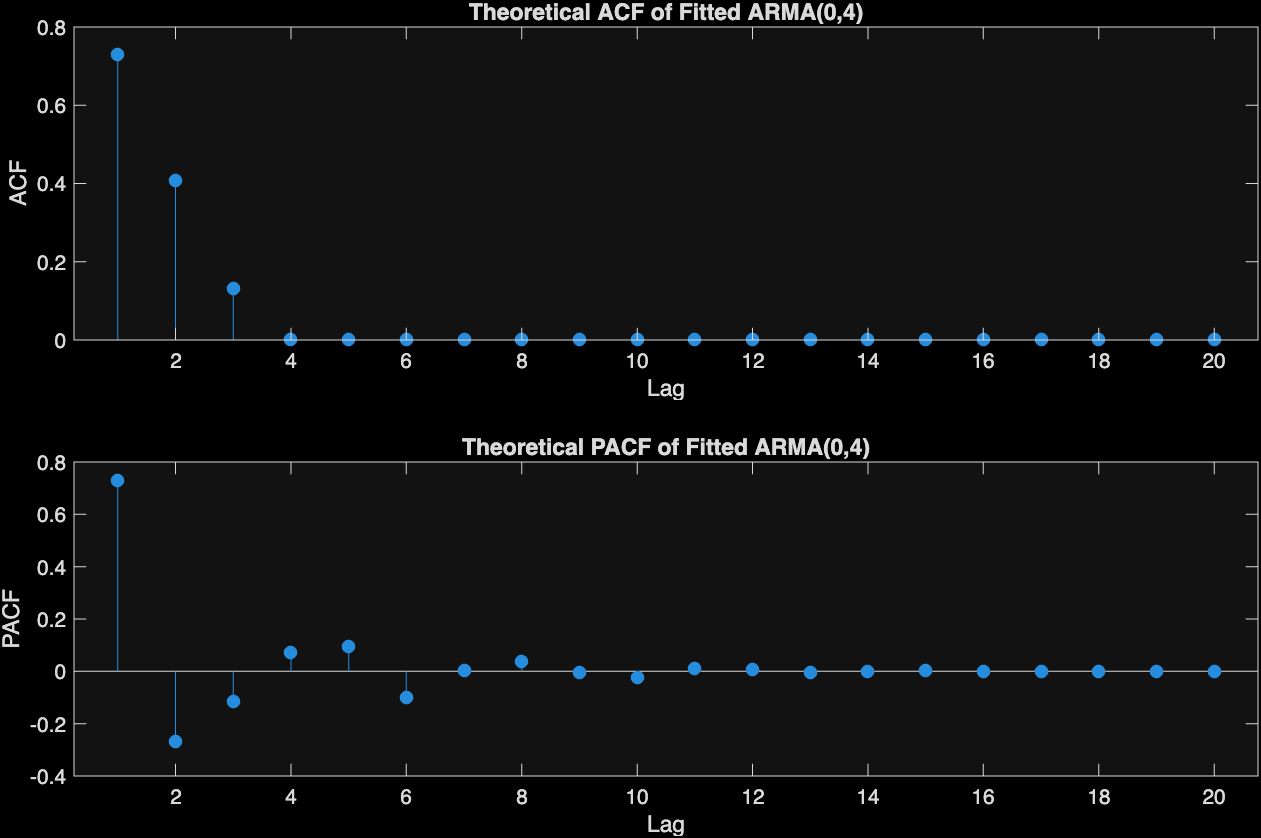
\includegraphics[width=0.6\textwidth]{ACVF.png} % Replace with your filename
    \caption{This is a caption for the figure}
    \label{fig:my_image}
\end{figure}
